\section{Vertex Reconstruction}\label{section:star_vertex}

In $pp$ collisions, where the charged-particle multiplicity is low, the vertex finding algorithm sometimes fails to find the~primary vertex. In addition, at high luminosity, vertex finder can fail due to the contribution of pile-up events and providing a wrong reconstructed vertex. In this study we required at least two reconstructed global tracks $n^\textrm{global}_\textrm{sel}\geq 2$ passing all the quality cuts listed in Sec~\ref{section:star_track_selection} but without $\textrm{DCA}_{xy}$ and $\textrm{DCA}_{z}$ cuts.  Additionally, MC events were accepted if the~$z$-coordinate of the true-level primary vertex was between $-80$ and $80$~cm. All corrections, described in this section, were calculated in three ranges of $\xi$ separately.

%\subsubsection{Track Quality Cuts Used for Vertexing}
The following quality cuts had to be passed by the global tracks used in the vertex reconstruction:
\begin{enumerate}
	\item Tracks must be matched with hits reconstructed in TOF,
	\item The number of the TPC hits used in the helix fit $N_\textrm{hits}^\textrm{fit}$ must be greater than 20,
	\item The ratio of the number of TPC hits used in the helix fit to the number of possible TPC hits $N_\textrm{hits}^\textrm{fit}/N_\textrm{hits}^\textrm{poss}$ must be greater than $0.52$,
	\item The transverse impact parameter with respect to the beamline $d_0$ must be less than 2 cm,
	\item The track's transverse momentum $p_\textrm{T}$ must be greater than $0.2$~GeV/c.
\end{enumerate}
 The~above track selection criteria are different than those used in the analysis. Thus, primary vertex reconstruction efficiency and fake vertex rate were calculated as a function of the~number of global tracks used in vertexing $n^\textrm{global}_\textrm{vrt}$ instead of $n^\textrm{global}_\textrm{sel}$. 

%\subsubsection{Vertex Efficiency and Fake Vertex Rate}
In the analysis exactly one vertex with $n_\textrm{sel}\geq 2$ is required.  The reconstructed vertex with the label \textit{best} is the one with the highest number of TOF-matched tracks. Since the fake vertices (not matched to the true-level primary vertex) are allowed in the analysis, the overall vertex-finding efficiency, $\epsilon_\textrm{vrt}\left(n_\textrm{vrt}^\textrm{global}\right)$, is expressed as:
\begin{equation}
\epsilon_\textrm{vrt}\left(n_\textrm{vrt}^\textrm{global}\right)=\epsilon_\textrm{vrt}^\textrm{best}\left(n_\textrm{vrt}^\textrm{global}\right)+\delta_\textrm{vrt}^\textrm{fake}\left(n_\textrm{vrt}^\textrm{global}\right)
\end{equation}
where:
\begin{description}
	\item $\epsilon_\textrm{vrt}^\textrm{best}\left(n_\textrm{vrt}^\textrm{global}\right)$ is the primary vertex reconstruction efficiency, determined as the ratio of the number of good reconstructed events (reconstructed best primary vertex with $n_\textrm{sel}\geq 2$) to the number of input MC events, where the reconstructed vertex is matched to the true-level primary vertex,
	\item $\delta_\textrm{vrt}^\textrm{fake}\left(n_\textrm{vrt}^\textrm{global}\right)$ is the fake vertex rate, determined as the ratio of the number of good reconstructed events (reconstructed best primary vertex with $n_\textrm{sel}\geq 2$) to the number of input MC events, where the reconstructed vertex is not matched to the true-level primary vertex.
\end{description}

The vertex-finding efficiency as a function of $n^\textrm{global}_\textrm{vrt}$ is shown in  Fig.~\ref{fig:vertexEffi}~(left). When there are exactly two global tracks used in the vertex reconstruction, $n^\textrm{global}_\textrm{vrt}=2$, the longitudinal distance between these tracks $|\Delta z_0|$  is used by the vertex-finding algorithm. Therefore, the vertex finding efficiency for such events $\epsilon_\textrm{vrt}\left(|\Delta z_0|\right)$ is given by:
\begin{equation}
\epsilon_\textrm{vrt}\left(|\Delta z_0|\right)=\epsilon_\textrm{vrt}^\textrm{best}\left(|\Delta z_0|\right)+\delta_\textrm{vrt}^\textrm{fake}\left(|\Delta z_0|\right)
\end{equation}
where: $\epsilon_\textrm{vrt}^\textrm{best}\left(|\Delta z_0|\right)$ is the primary vertex reconstruction efficiency, $\delta_\textrm{vrt}^\textrm{fake}\left(|\Delta z_0|\right)$ is the fake vertex rate.

Figure~\ref{fig:vertexEffi}~(right) shows the vertex finding efficiency for events with $n^\textrm{global}_\textrm{vrt}=2$. This efficiency is smaller than $20\%$ for tracks with $|\Delta z_0|>2$~cm, hence the analysis was limited to  events with  $|\Delta z_0|<2$~cm, when $n^\textrm{global}_\textrm{vrt}=2$. 
\begin{figure}[h!]
	\centering
		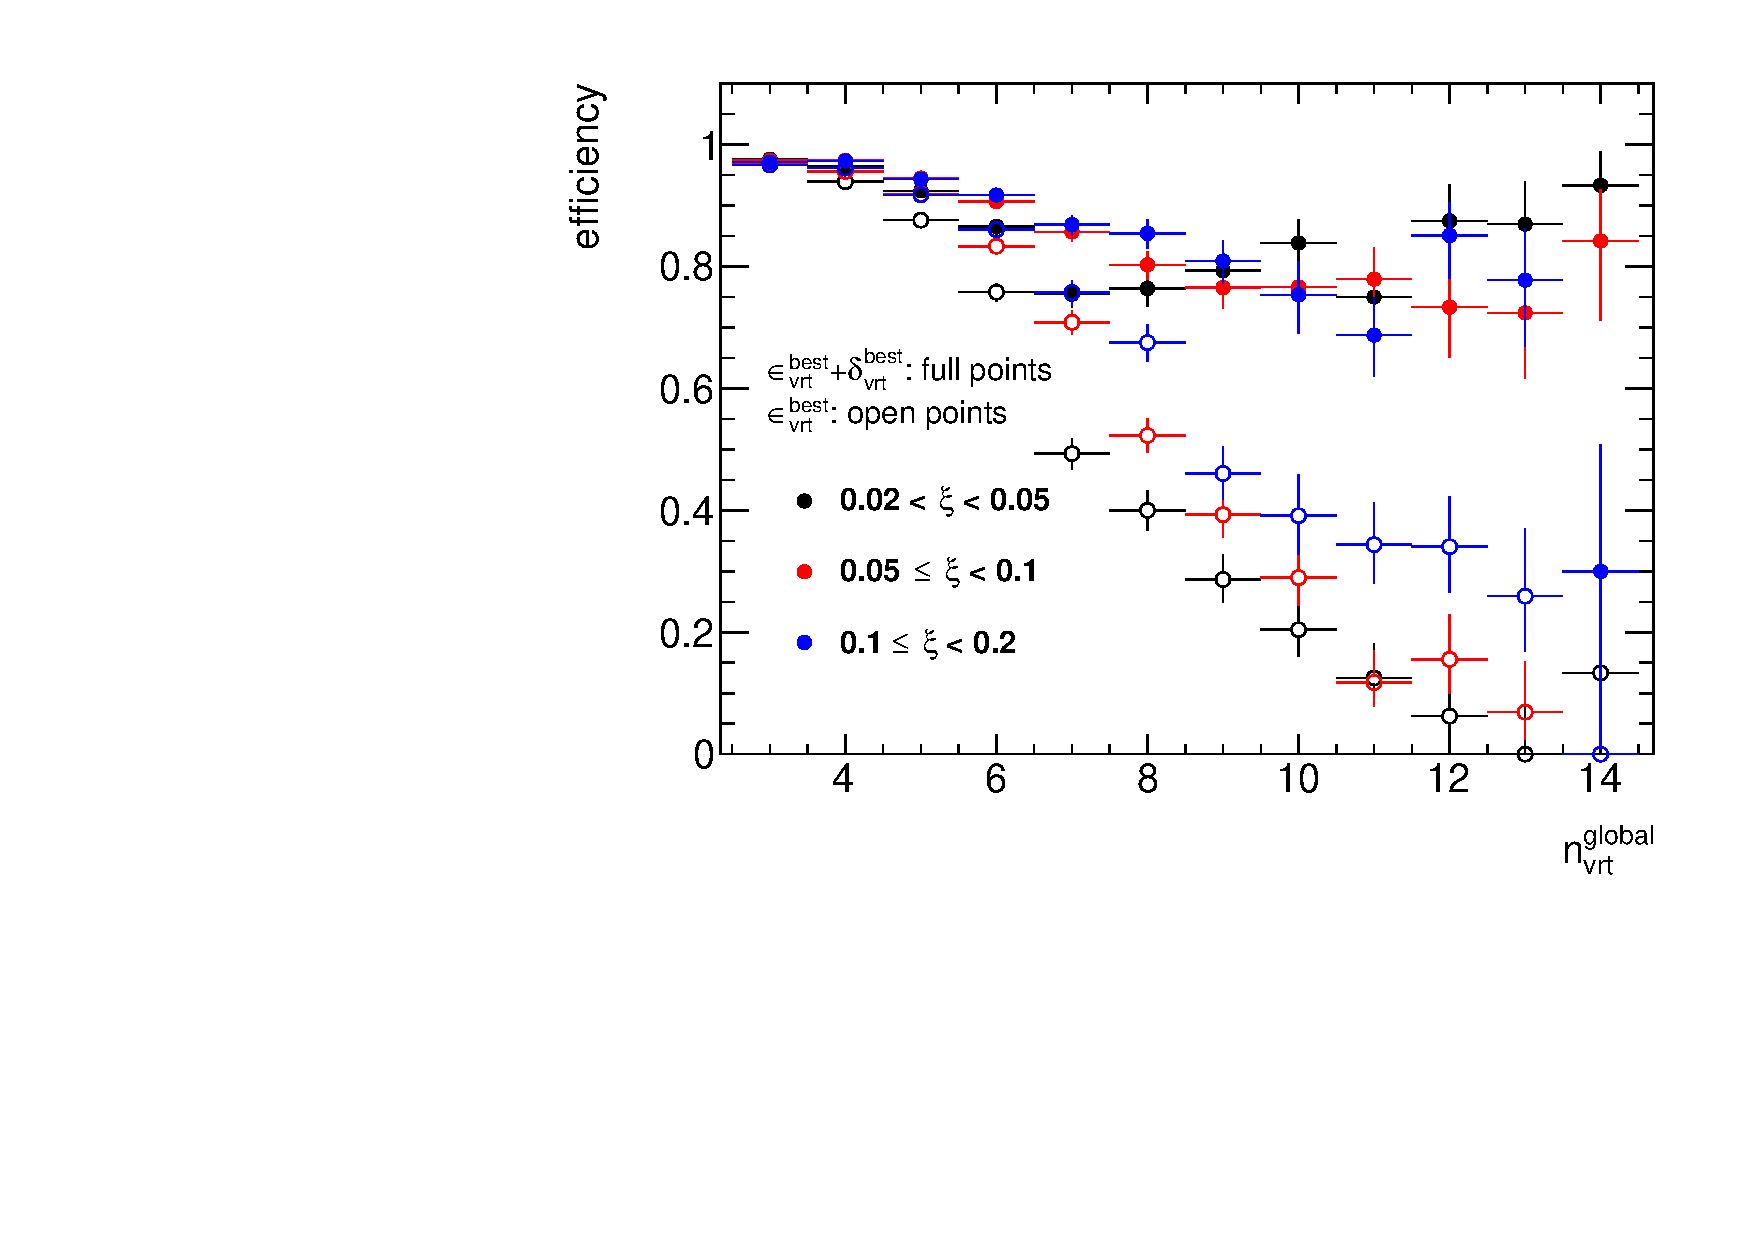
\includegraphics[width=0.49\textwidth,page=1]{chapters/chrgSTAR/img/vertex/vertexEffi_ksi.pdf}
		\includegraphics[width=0.49\textwidth,page=8]{chapters/chrgSTAR/img/vertex/vertexEffi_ksi.pdf}
		\caption{Vertex-finding efficiency in three ranges of $\xi$ as a function of  (left) $n^\textrm{global}_\textrm{vrt}$ and (right) with respect to the $|\Delta z_0|$ between reconstructed tracks in events with $n^\textrm{global}_\textrm{vrt}=2$. }
		\label{fig:vertexEffi}
\end{figure}

%\subsubsection{Other Corrections to the Reconstructed Vertices}
Events with reconstructed best vertex are rejected if there  are:
\begin{enumerate}[label=\alph*)]
	\item more than one additional TOF vertices,
	\item additional secondary TOF vertex from interactions with the detector dead-material,
	\item additional fake TOF vertex,
	\item additional primary TOF vertex (vertex splitting or background vertex reconstructed as best vertex),
	\item additional decay TOF vertex.  
\end{enumerate}
The correction for vetoing such events, $\epsilon_\textrm{vrt}^\textrm{veto}\left(n_\textrm{vrt}^\textrm{global}\right)$, is given by: 
\begin{equation}
\begin{split}
\epsilon_\textrm{vrt}^\textrm{veto}\left(n_\textrm{vrt}^\textrm{global}\right) & =1-\frac{\textrm{number of events with more than one reconstructed  TOF vertex}}{\textrm{number of events with at least one reconstructed TOF vertex}} \\
& =1-\epsilon_a-\epsilon_b-\epsilon_c-\epsilon_d-\epsilon_e
\end{split}
\end{equation}
where $\epsilon_a-\epsilon_e$ are the fractions of events with additional vertices, whose labels  are listed above.% shown in \ref{fig:vertexVeto}.

As before, the correction was calculated as a function of $|\Delta z_0|$ for events with $n^\textrm{global}_\textrm{vrt}=2$. Figure~ \ref{fig:vertexVeto} shows the fraction of multi-vertex events  with respect to the $n_\textrm{vrt}^\textrm{global}$. There is a~large fraction of events ($>50\%$) with additional background vertices for $n_\textrm{vrt}^\textrm{global}\geq 9$, what would result in large correction factor. Hence, the analysis was limited to events with $n_\textrm{sel}\leq8$. On the other hand,  the total fraction of multi-vertex events, $\epsilon_a+\epsilon_b+\epsilon_c+\epsilon_d+\epsilon_e$, as a function of $|\Delta z_0|$, shown in Fig.~\ref{fig:vertexVetoDZ}, demonstrates that $\epsilon_\textrm{vrt}^\textrm{veto}(|\Delta z_0|)$ is very large ($>98\%$) for events with $n^\textrm{global}_\textrm{vrt}=2$.
\begin{figure}[h!]
	%\vspace{-0.5cm}
	\centering
	\begin{subfigure}{.47\textwidth}
		\includegraphics[width=\textwidth,page=9]{chapters/chrgSTAR/img/vertex/vertexEffi_ksi.pdf}
	\end{subfigure}
	\begin{minipage}{.47\textwidth}
		\caption{Total fraction of multi-vertex events as a function of $|\Delta z_0|$ for events with $n^\textrm{global}_\textrm{vrt}=2$  in three ranges of $\xi$.}
		\label{fig:vertexVetoDZ}
	\end{minipage}
	\vspace{-0.5cm}
\end{figure}
\begin{figure}[h!]
	%\vspace{-0.5cm}
	\centering
	\begin{subfigure}{.47\textwidth}
		\includegraphics[width=\textwidth,page=3]{chapters/chrgSTAR/img/vertex/vertexEffi_ksi.pdf}
	\end{subfigure}
	\begin{subfigure}{.47\textwidth}
		\includegraphics[width=\textwidth,page=4]{chapters/chrgSTAR/img/vertex/vertexEffi_ksi.pdf}
	\end{subfigure}
	\begin{subfigure}{.47\textwidth}
		\includegraphics[width=\textwidth,page=5]{chapters/chrgSTAR/img/vertex/vertexEffi_ksi.pdf}
	\end{subfigure}
	\begin{subfigure}{.47\textwidth}
		\includegraphics[width=\textwidth,page=6]{chapters/chrgSTAR/img/vertex/vertexEffi_ksi.pdf}
	\end{subfigure}
	\begin{subfigure}{.47\textwidth}
		\includegraphics[width=\textwidth,page=7]{chapters/chrgSTAR/img/vertex/vertexEffi_ksi.pdf}
	\end{subfigure}
	\begin{minipage}{.47\textwidth}
			\caption{Fraction of multi-vertex events  with respect to the $n_\textrm{vrt}^\textrm{global}$ in three ranges of $\xi$. Each contribution is shown separately: (top left) more than one additional vertices, (top right) additional secondary vertex from the interactions with the detector dead-material, (middle left) additional fake vertex, (middle right) additional primary vertex and (bottom) additional decay vertex.}
			\label{fig:vertexVeto}
	\end{minipage}
	%\vspace{-1.5cm}
\end{figure}


%\FloatBarrier
